\newcommand\myeq{\mkern1.5mu{=}\mkern1.5mu}


In this section we will discuss the optimization results of both wind farms, the apparent benefit of coupled turbine layout and design optimization, as well as the benefit of heterogeneous turbine design in a wind farm.
We first present results from the 32-turbine circular wind farm optimizations and then compare to the 60-turbine Princess Amalia wind farm optimizations. 


\subsection{Circular Wind Farm}

Figure \ref{circular_results} shows the optimal COE results for the circular wind farm. As shown in the legends, the white points represent a layout-only optimization with the baseline turbine design, the gray indicate a sequential-turbine-design-then-layout optimization, the black squares show a coupled-turbine-design-and-layout optimization, and the half blue and pink points represent a coupled-design-and-layout optimization with two turbine groups.  As expected, the general trends for all optimization runs show that the higher wind speed from high wind shear results in a lower, superior optimal COE. Additionally, the widely spaced wind turbines indicated by the larger spacing multipliers also result in lower COE due to less wake interaction between turbines. We will discuss each of these optimizations in detail below.


\begin{figure}[htbp]
  \centering
  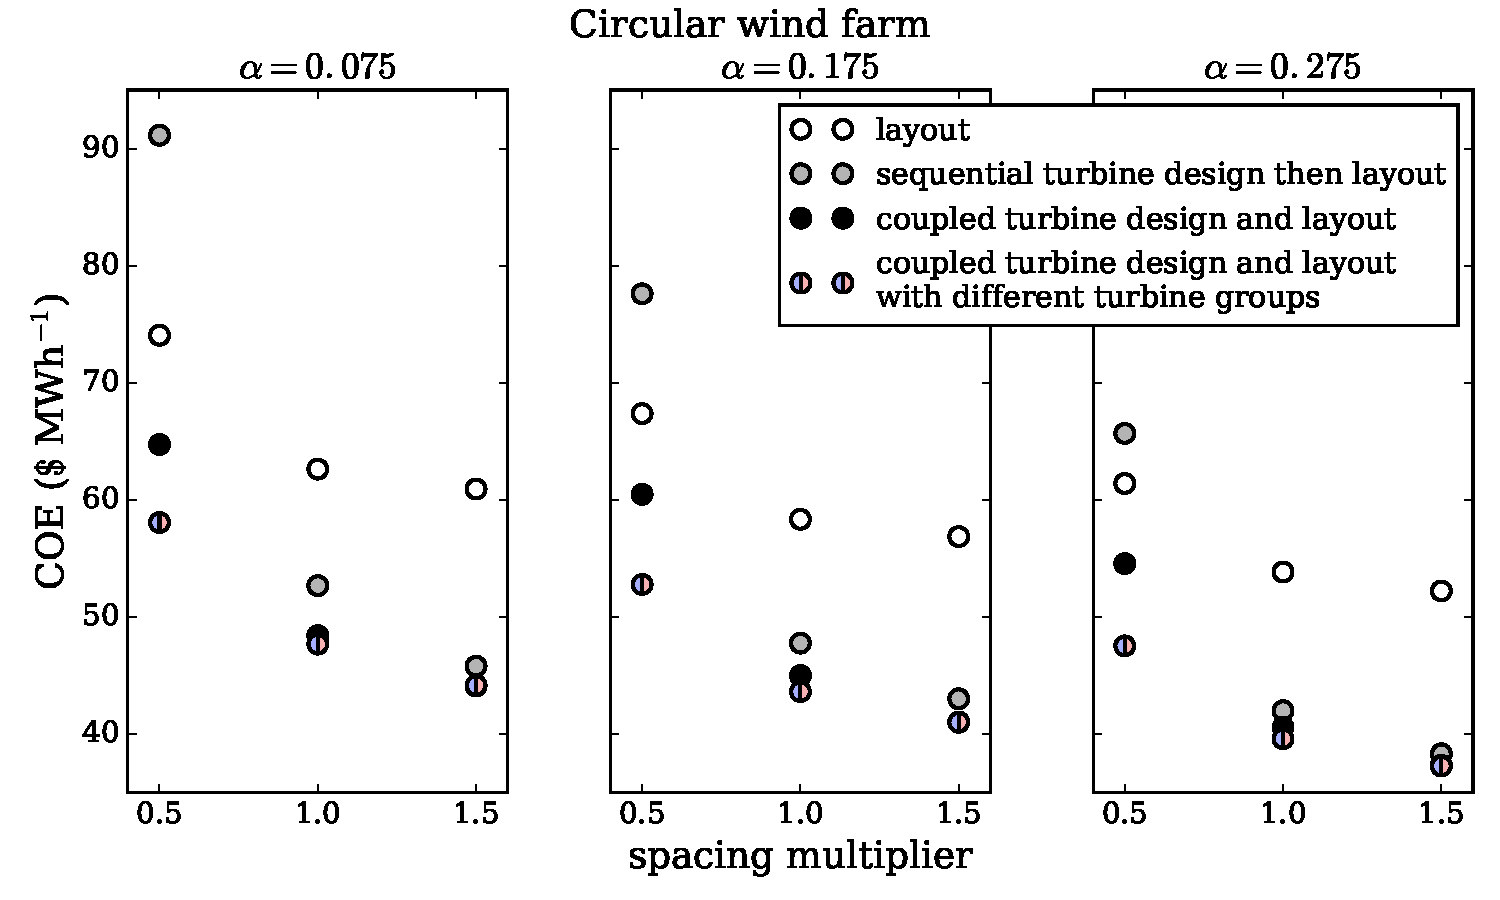
\includegraphics[width=0.7\textwidth]{Figures/circular_results1.pdf}
  \caption{\label{circular_results} The optimal COE results for the circular wind farm layout with 32 turbines. Each of the subfigures corresponds to optimization runs with a different shear exponent, from left to right $\alpha=0.075,0.175,0.275$. Within each subfigure, the x axis shows the size of the wind farm based on the spacing multiplier, from left to right $\beta=0.5,1.0,1.5$. The different points represent the layout optimization with the baseline turbine design, sequential-turbine-design-then-layout optimization, coupled-layout-and-turbine-design optimization with homogeneous turbine design throughout the farm, and layout-and-turbine-design optimization with two different turbine design groups.}
\end{figure}



\subsubsection{Circular Wind Farm: Sequential-Turbine-Design-then-Layout Optimization}
The gray dots in Fig. \ref{circular_results} show the optimal COE results for a sequential optimization. First, a turbine was designed for minimal COE in isolation with the free stream wind conditions. This turbine design was then used in a wind farm where the layout was subsequently optimized. 
The rotor diameter was constrained such that the turbine spacing constraints would be satisfied in the baseline farm where the turbine would be installed. This was only applicable for the smallest wind farms, where $\beta=0.5$. 
For each shear exponent, the optimal turbine design was the maximum rotor diameter and turbine rating allowed by the optimizer. The rotor diameter was constrained by the spacing constraint for $\beta=0.5$, and by the bound constraint for other turbine spacings.
Figure \ref{circular_turbines_seq} shows the optimal isolated turbine designs for each shear exponent and spacing multiplier, as well as the baseline turbine design. Because these turbines are optimized in isolation and the spacing constraint was not active, the designs for $\beta=1.0,1.5$ are the same. 
When these optimized turbine designs are used in each wind farm instead of the baseline turbine design, there is a large COE improvement for the spacing multipliers of $\beta=1.0, 1.5$. For $\beta=1.0$, COE decreases 15.9--22.0\% compared to an optimized wind farm with the baseline turbine design. For $\beta=1.5$ the COE decrease is even larger, 24.8--26.6\% across all shear exponents. 
For the smallest wind farm, $\beta=0.5$, the turbine design optimized in isolation results in an extremely inefficient wind farm. When in the wind farm environment, exposed to much lower average wind speeds, this design results in a COE that is much worse than the baseline turbine design. The expense from a bigger and taller turbine, coupled with the strong wake interactions among turbines that are so closely spaced means that for this wind farm, optimizing the turbine in isolation actually decreases the wind farm performance. 


\begin{figure}[htbp]
  \centering
  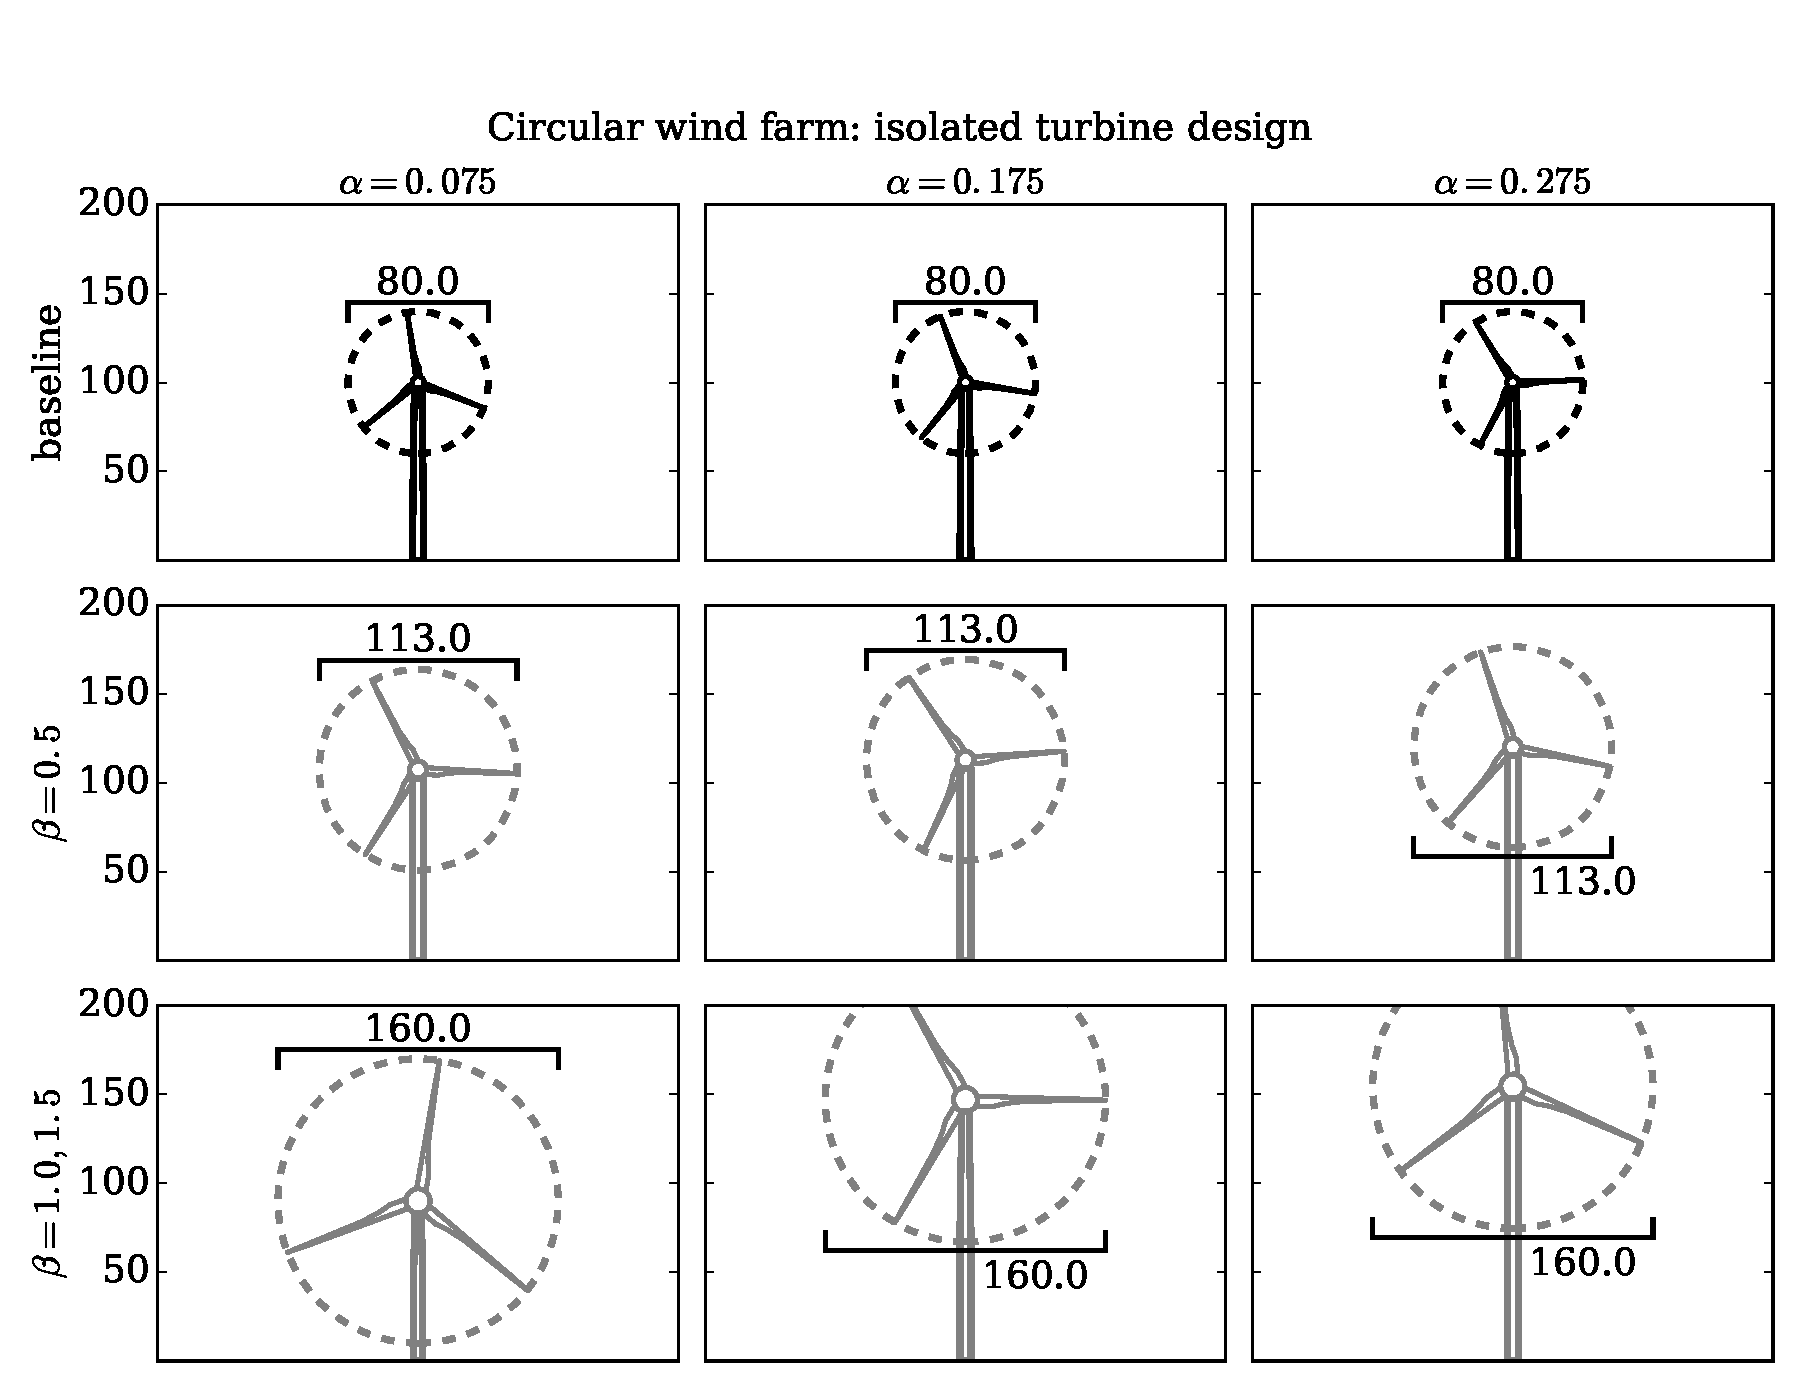
\includegraphics[trim={0.5cm 0.3cm 0.3cm 2.75cm},clip,width=0.7\textwidth]{Figures/turbineSizesCircular_sequential.pdf}
  \caption{\label{circular_turbines_seq} The optimal turbine heights and rotor diameters for the isolated turbine design optimization for the circular farm wind conditions. These designs were then used in the sequential turbine-design-then-layout optimizations. The columns, from left to right, show the turbines optimized for $\alpha=0.075,0.175$, and $0.275$. The rows, from top to bottom, show the baseline turbine design, the turbine optimized for the small wind farm ($\beta=0.5$), and the turbine designs for the larger wind farms ($\beta=1.0,1.5$)}
\end{figure}



\subsubsection{Circular Wind Farm: Coupled-Turbine-Design-and-Layout Optimization}
Next we will discuss the optimization results of the coupled turbine-design-and-layout optimizations, represented by the black squares in Fig. \ref{circular_results}. For every shear exponent and spacing multiplier, there is a large benefit to performing the coupled turbine-design-and-layout optimization compared to the layout-only optimization with the baseline turbine design. Additionally, and more importantly, the coupled optimization results in appreciably lower COE than the sequential design-then-layout optimization. Obviously for a spacing multiplier of $\beta=0.5$, the coupled optimization is far superior to the sequential simply by being better than the baseline turbine design. For the spacing multiplier of $\beta=1.0$, 
compared to the sequential optimizations, coupled optimization results in an additional 6.82\%, 4.75\%, and 2.65\% COE improvement from layout only optimization for shear exponents $\alpha=0.075, 0.175,$ and $0.275$, respectively. For the largest wind farm, $\beta=1.5$, the coupled optimization results in an additional 2.78\%, 3.50\%, and 1.88\% COE improvement compared to the sequential case. 

There are several conclusions we can make from both the sequential and coupled turbine design and layout optimizations. First, and most apparent, optimizing turbine design results in a much better wind farm than a farm in which the turbines are selected arbitrarily or a priori. Second, and more importantly, optimizing turbine design coupled with the turbine layout is significantly better than optimizing the turbine design for the free stream wind conditions alone. In a wind farm, turbines rarely experience the free stream wind conditions as they are often waked by the other turbines in the farm. Therefore, the optimal turbine design is based on on average slower wind speeds than the free stream wind. This results in turbines with smaller hub heights, rotor diameters, and rated powers. 
%
One could conceivably optimize the turbine design for some wind speed slower than the free stream and closer to the average speed in the wind farm, which would likely be better than optimizing the turbine design for the free stream wind speed. However, the average wind speed in a farm is dependent on the turbine layout, making it difficult to choose the correct speed for which to design the turbines. Thus, is important to couple the turbine design and layout optimization for a superior wind farm. 

Figure \ref{circular_turbines_1} shows the optimal rotor diameters and hub heights for the coupled turbine design and layout optimizations. For a spacing multiplier $\beta=0.5$, the turbines are very close together and in general are heavily waked. Thus to satisfy spacing constraints and because the average wind speed is very low, the optimal rotor diameter is small: about 90 meters. When the turbines are spaced farther apart, shown for the larger spacing multipliers, the optimal rotor diameter is much larger: closer to 120--130 meters. In these farms, wake interactions are not as severe, meaning that the extra power production from larger rotors is worth the extra turbine capital cost. Also notice the trend of the optimal turbine height with wind shear exponent; for a low wind shear exponent, $\alpha=0.075$, the wind speed does not drastically change with height (see Fig. \ref{shear_profile}). Therefore, for this wind condition it is desirable to have short hub heights with a lower turbine capital cost. For the higher shear exponents, $\alpha=0.175,0.275$, the wind speed increases much more with height (See Fig. \ref{shear_profile}). In these cases, for every spacing multiplier, the extra cost of building the taller turbines is made up for in the additional power produced from the high wind speeds. Remember that a larger rotor diameter reduces the relative spacing between turbines in the farm, as the original spacing was based on a diameter of 80 meters.

\begin{figure}[htbp]
  \centering
  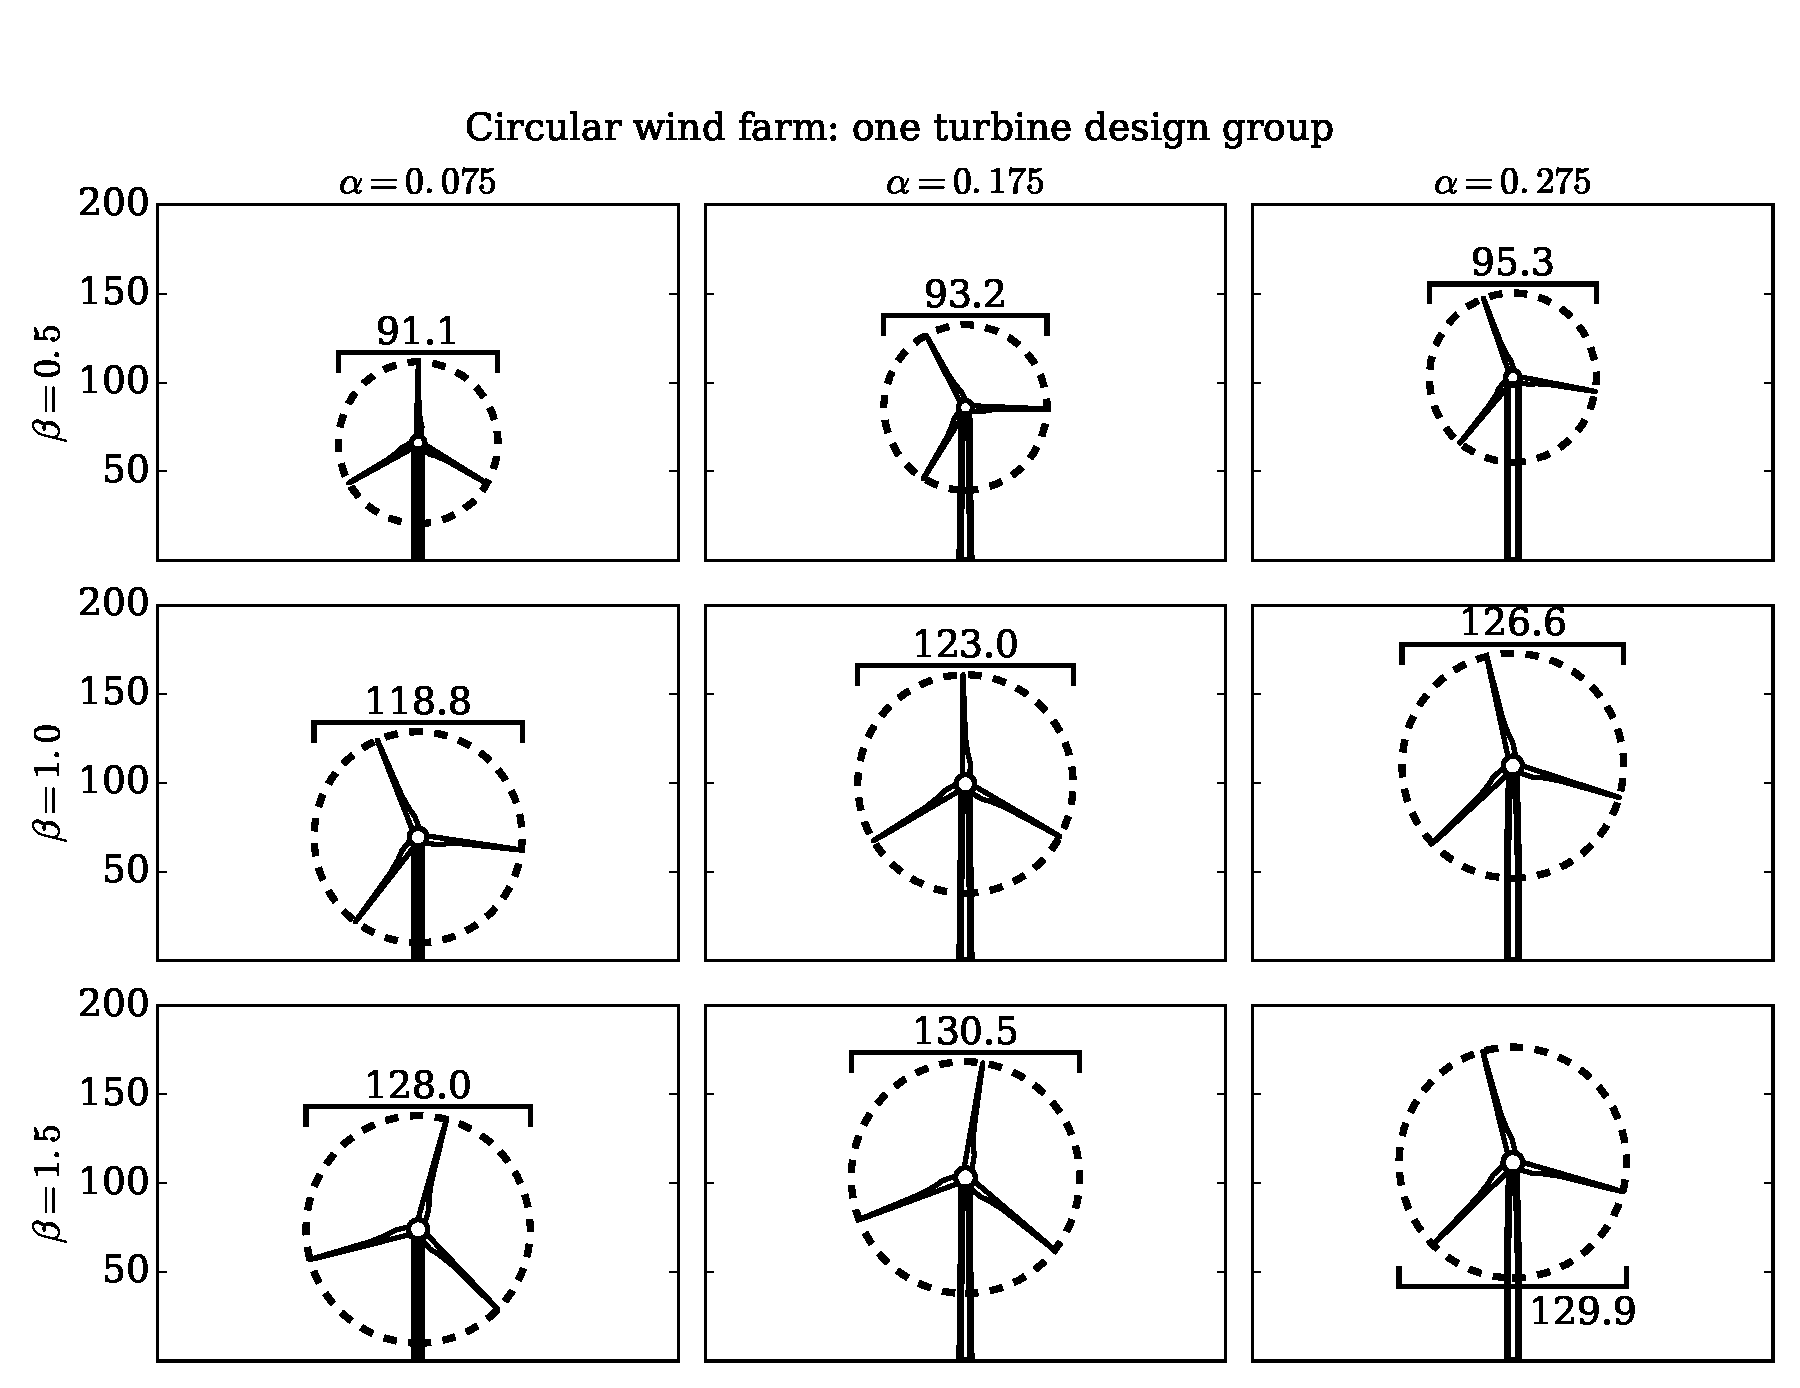
\includegraphics[trim={0.5cm 0.3cm 0.3cm 2.75cm},clip,width=0.7\textwidth]{Figures/turbineSizesCircular_1.pdf}
  \caption{\label{circular_turbines_1} The optimal turbine heights and rotor diameters for the optimization runs with coupled layout and turbine design with homogeneous turbine design throughout the circular wind farm. Each column shows a different shear exponent, with $\alpha=0.075,0.175,0.275$ from left to right. Each row shows a different farm spacing multiplier, with $\beta=0.5,1.0,1.5$ from top to bottom.}
\end{figure}


In Fig. \ref{circular_power}, the black points show the optimal rated powers for the turbines in each optimization case. The optimal rated power scales with the turbine rotor diameter and hub height. Higher turbine rating is expensive, therefore the small rotors and short turbines, which are more heavily waked and don't produce as much power, do not require a large power rating. The extra cost is not justified by a very slight increase in power. For the high shear exponents and spacing multipliers, the turbines are exposed to faster wind speeds. These turbines are bigger and taller, and the extra power production from raising the rated power is worth the additional cost.


\begin{figure}[htbp]
  \centering
  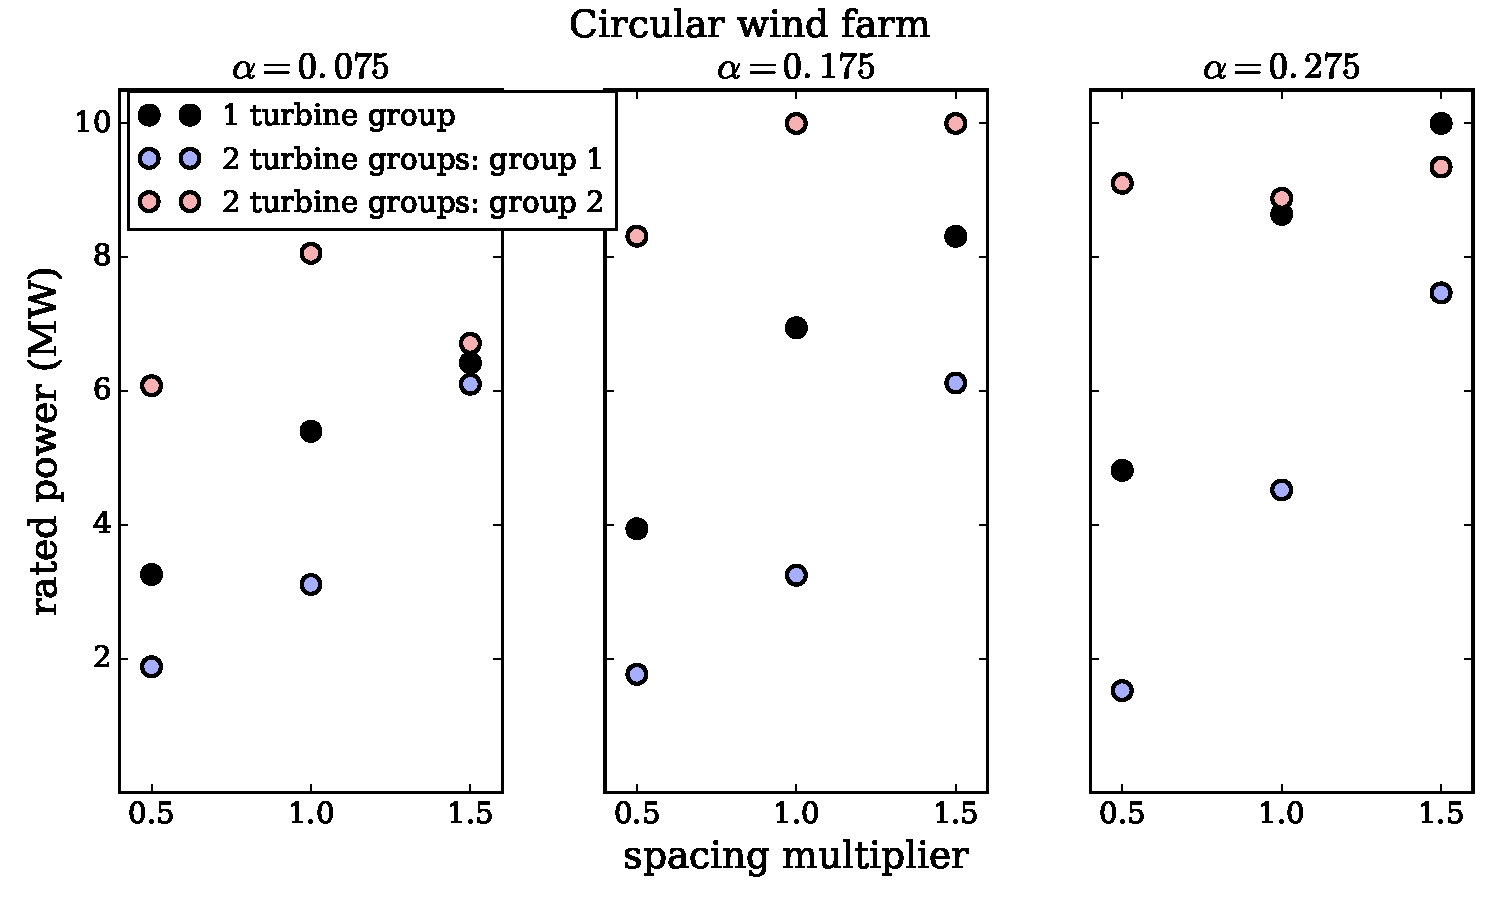
\includegraphics[trim={0.5cm 0.3cm 0.3cm 0.75cm},clip,width=0.7\textwidth]{Figures/circlePowers.pdf}
  \caption{\label{circular_power} The optimal rated powers for the circular wind farm for the optimization runs with coupled layout and turbine design for both uniform wind farm turbine design and with two different turbine design groups. The three subfigures show a different shear exponent, with $\alpha=0.075,0.175,0.275$ from left to right. within each subfigure, the x axis shows different farm spacing multipliers, with $\beta=0.5,1.0,1.5$ from left to right.}
\end{figure}



\subsubsection{Circular Wind Farm: Coupled Turbine Design and Layout Optimization with Two Turbine Groups}

Now we will discuss the most interesting case, the coupled-turbine-design-and-layout optimization with two different turbine groups. The optimal COE results of these optimizations are shown with the blue and pink points in Fig. \ref{circular_results}. Most visibly, for the smallest spacing multiplier, $\beta=0.5$, there is a large COE improvement for the heterogeneous turbine design optimizations compared to the farms with homogeneous turbine design (shown by the black squares in Fig. \ref{circular_results}). For this spacing multiplier, the heterogeneous turbine design farms reduce COE by 21.6\%, 21.67\%, and 22.6\% compared to the layout-only optimization for shear exponents of $\alpha=0.075,0.175$, and $0.275$, respectively. The coupled optimizations with one turbine group reduce COE by 12.59\%, 10.24\%, and 11.15\%. For the smallest spacing multiplier, optimizing turbine design and layout with two turbine groups reduces COE by an additional 9--11.45\% compared to just one turbine group. For the spacing multiplier $\beta=1.0$, the coupled optimization with two turbine groups results in an additional 1.16--2.35\% COE decrease compared to with one turbine group. This is much smaller than the more tightly packed wind farms, but still non-negligible. For the spacing multiplier $\beta=1.5$, the optimization with two turbine groups results in only an additional 0--0.12\% COE decrease, indicating that when the turbines are spread very far apart there is no benefit to allowing multiple turbine designs in the same farm.

The two different rotor designs in the same wind farm help to improve COE by reducing the wake interaction between wind turbines. By combining tall and short turbines, with large and small rotor sizes, there are more dimensions that the optimizer can manipulate to avoid wakes and improve performance. For the tightly packed wind farms, the turbine layout is greatly limited by the turbine spacing constraints. Additionally, as the turbines are closer together, the wakes greatly reduce the wind speed as they have not had an opportunity to mix with the free steam air. Both of these factors mean there is a large benefit to avoiding the wakes of other turbines by any means possible. For the larger wind farms where the turbines are spaced farther apart, the wakes are not as detrimental and there is more area in which to avoid wakes in the horizontal plane without needing to change hub height or rotor diameter. In these cases, the heterogeneous turbine designs are not as beneficial.

Figure \ref{circular_turbines} shows the optimal rotor diameter and hub height of each turbine group for these cases of coupled turbine design and layout optimization with two different groups. For the spacing multiplier $\beta=0.5$, when the turbines are very close together, there is a large difference in both the rotor diameter and hub height of each turbine group. Group 1 is extremely small and short, smaller than even the baseline rotor diameter, while group 2 is much larger. Even if turbines from each group were immediately adjacent to each other, there would be minimal wake interaction between the turbines. For the small wind farms, the sacrifice in power that comes from one very small and short turbine is made up for in the decreased wake interference between turbine groups. Essentially, having two different turbine groups doubles the effective spacing between turbines, because turbines in different groups do not affect each other. For a larger spacing multiplier of $\beta=1.0$, each turbine group is still remarkably different in size and height. The turbines are larger than they were for the smallest wind farm because the average wind speed is faster when the turbines are spread farther apart. Notice that, compared to the optimized turbines for $\beta=0.5$, the smaller turbines when $\beta=1.0$ are larger and overlap more with the taller, bigger turbines. In this case, the power increase from bigger rotor diameters outweighs the benefit gained from reducing wake interference. 

The turbine sizes for the largest wind farm, $\beta=1.5$, demonstrate the multi-modality of the wind farm optimization problem. For this spacing multiplier, each turbine group is more similar than in the previous wind farm sizes. For the lowest shear exponent, $\alpha=0.075$, both turbine groups are almost identical. For $\alpha=0.175,0.275$, there is some difference in each rotor diameter and hub height, although the difference is not as pronounced as it was for the smaller wind farms. However, Fig. \ref{circular_results} shows that for $\beta=1.5$ the optimal COE from coupled turbine design and layout optimization is the almost exactly the same with one and two turbine groups. So, a wind farm with the homogeneous turbine design shown in the bottom row of Fig. \ref{circular_turbines_1}, and a wind farm with two different turbine designs shown in the bottom row of Fig. \ref{circular_turbines} result in a very similar optimal COE. The same optimal result is achieved with drastically different farms, each with different turbines and layouts.  

\begin{figure}[htbp]
  \centering
  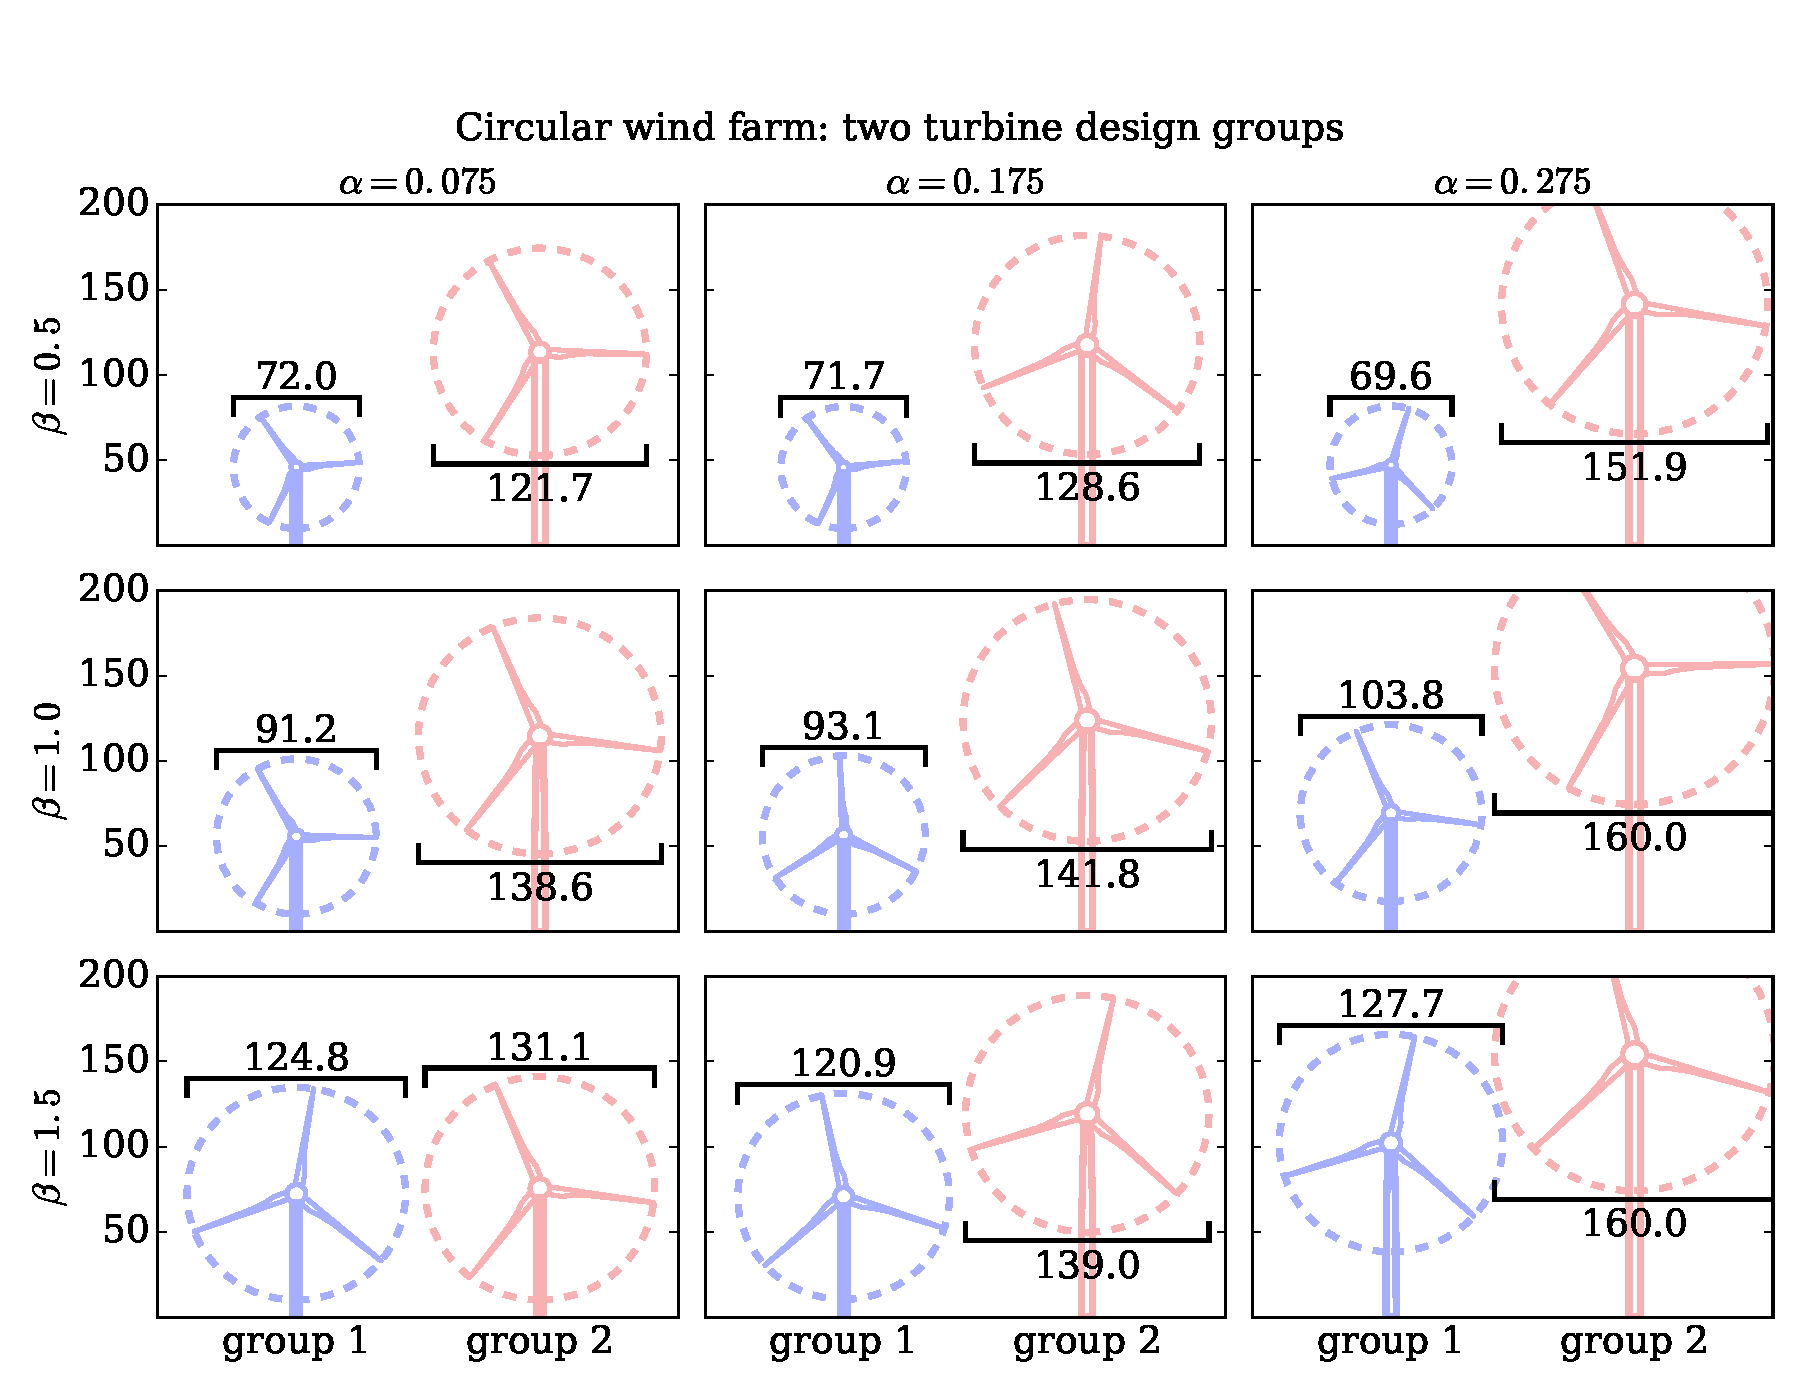
\includegraphics[trim={0.5cm 0.3cm 0.3cm 2.75cm},clip,width=0.7\textwidth]{Figures/turbineSizesCircular_2.pdf}
  \caption{\label{circular_turbines} The optimal turbine heights and rotor diameters for the optimization runs with coupled layout and turbine design with two different turbine design groups for the circular wind farm. Each column shows a different shear exponent, with $\alpha=0.075,0.175,0.275$ from left to right. Each row shows a different farm spacing multiplier, with $\beta=0.5,1.0,1.5$ from top to bottom.}
\end{figure}


Figure \ref{circular_power} shows the optimal rated power of each height group for the optimization cases with two different turbine groups. The blue and pink dots in this plot correspond to the turbines of the same color in Fig. \ref{circular_turbines}. As with the homogeneous turbine wind farm, the optimal rated power scales with the optimal turbine height and diameter. These larger, taller turbines are optimal in wind farms where they will be exposed to high wind speeds and produce large amounts of power. From a power production standpoint, it is undesirable to ever have a turbine's power limited by the rating. However, turbines with high ratings are more expensive, and not worth the cost if the turbine is generally producing low amounts of power. Therefore, the short, small turbines are optimal with a low, cheap power rating. The larger, taller turbines which produce much more electricity utilize the higher ratings.





\subsection{Princess Amalia Wind Farm Results}

In this section, we will discuss the results from the Princess Amalia wind farm optimizations.
All of the optimizations that were performed with the circular, 32-turbine wind farm were repeated for the larger, 60-turbine Princess Amalia wind farm. We will show and briefly discuss the optimal COE results; however, the optimal turbine designs for the Princess Amalia wind farm optimizations were very similar to those for the circular wind farm and therefore will not be included in this paper.

Figure \ref{amalia_results} shows the COE results for the 60-turbine Princess Amalia wind farm optimizations.  The trends are similar to the smaller, circular wind farm. Coupled turbine design and layout optimization is superior to optimizing each sequentially, especially for the smaller wind farms where the wind speeds are much lower than the free stream. For the farms with closely spaced wind turbines, two different turbine designs in the same farm are significantly better than the farms optimized with a homogeneous turbine design. If the largest wind farms ($\beta=1.5$) benefit from two different turbine design groups, that benefit is negligible. The optimal COE values for the Princess Amalia wind farm are slightly lower across the board than the circular wind farm COE values. This is partly because there are more turbines in the Princess Amalia wind farm so a smaller portion of the total cost comes from overhead but also is partly due to the Princess Amalia wind turbines being spaced slightly farther apart than those in the circular wind farms. Another major difference between the optimal COE values of each wind farm is in the optimization case with two turbine design groups. For the Princess Amalia wind farm and a spacing multiplier of 0.5, two turbine groups provides and additional COE decrease of 6.13--9.11\% compared to the wind farm with homogeneous turbine design. This is significant; however, it is not as large as the 9.01--11.45\% additional COE decrease in the circular wind farm optimizations for the same spacing multiplier. Again, the main cause of this seems to be that the turbines in the circular wind farms are slightly closer together than the turbines in the Princess Amalia wind farms.


\begin{figure}[htbp]
  \centering
  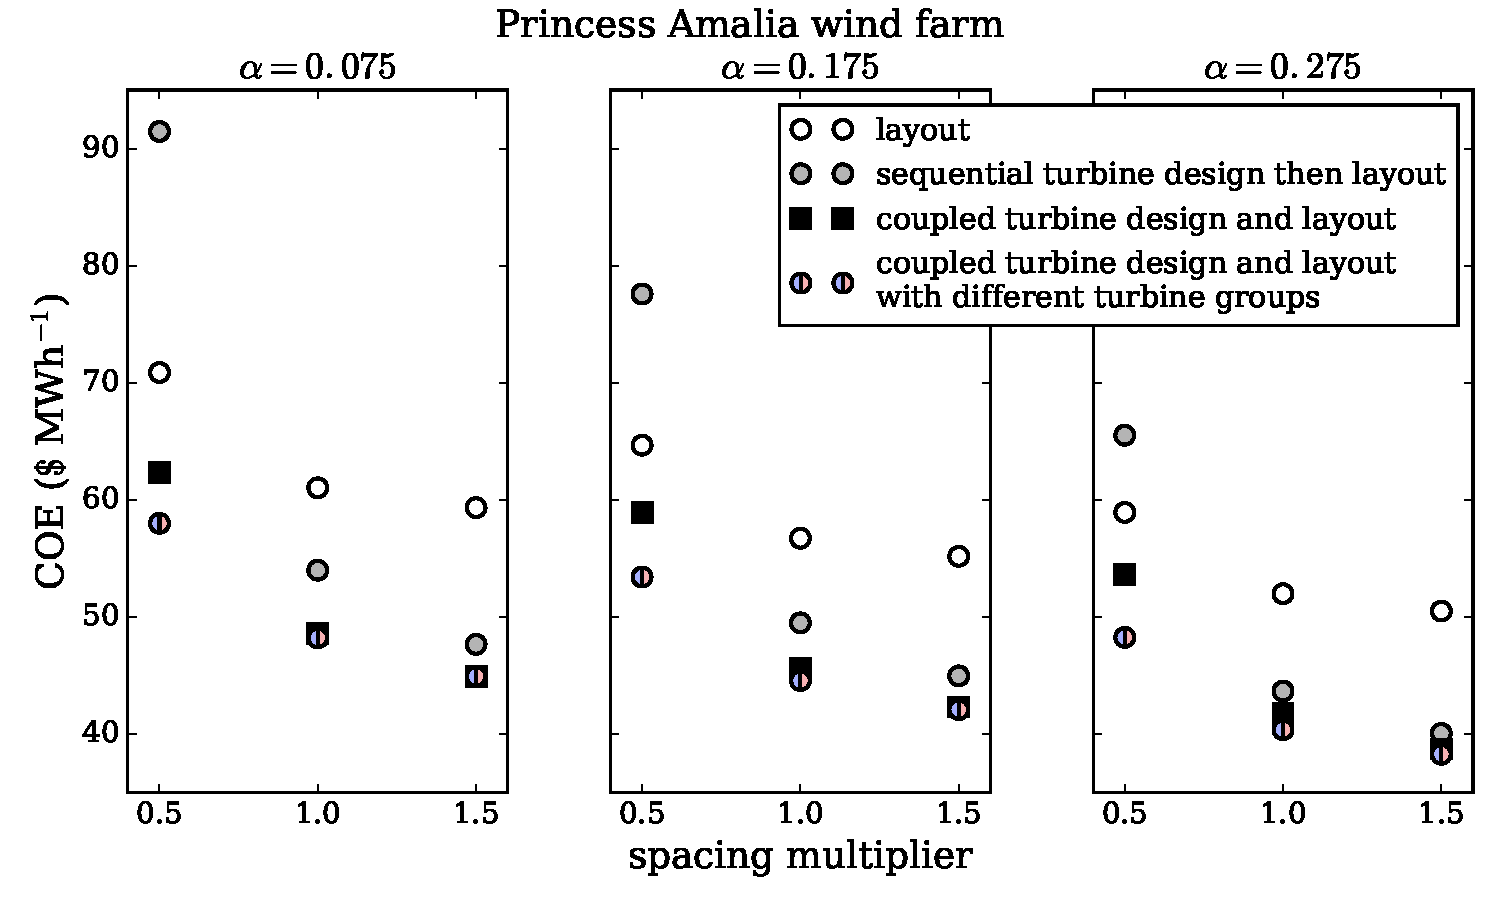
\includegraphics[width=0.7\textwidth]{Figures/amalia_results1.pdf}
  \caption{\label{amalia_results} The optimal COE results for the Princess Amalia wind farm layout with 60 turbines. Each of the subfigures corresponds to optimization runs with a different shear exponent, from left to right $\alpha=0.075,0.175,0.275$. Within each subfigure, the x axis shows the size of the wind farm based on the spacing multiplier, from left to right $\beta=0.5,1.0,1.5$. The different points represent the layout optimization, sequential turbine-design-then-layout optimization, coupled layout-and-turbine-design optimization with homogeneous turbine design throughout the farm, and layout-and-turbine-design optimization with two different turbine design groups.}
\end{figure}



Table \ref{results_table} shows how the optimal COE results for each wind farm compared to the layout optimization with the baseline wind turbine design. These numbers compare the relative benefit of performing turbine design with the various scenarios mentioned. High numbers represent a large COE decrease compared to the layout-only optimization for a given shear exponent and spacing multiplier combination; they do not necessarily represent a low COE.
There are a few interesting numbers in this table. Most obviously is the negative values (shown in red) for the sequential optimization with a spacing multiplier of 0.5. For these farms, sequential optimization is actually worse than the baseline. Also notice the COE decrease from coupled optimization with one group to two groups. For $\beta=0.5$, there is a huge benefit to having two groups, for $\beta=1.0$ there is a small benefit, and for $\beta=1.5$ there is no benefit at all. Finally, the benefit of coupled optimization with one group compared to sequential optimization is important. Again, there is a huge benefit to coupled optimization for the smallest spacing multiplier, and this relative benefit decreases as the wind farm size grows. However, even for $\beta=1.5$, there is an appreciable benefit to coupled design-and-layout optimization compared to sequential.



\begin{center}
\begin{table}
\caption{The percent COE decrease of the various optimization cases with respect to layout-only optimization. This table does not show the overall desirability of the optimal wind farm, but the relative improvement of different considerations of turbine design optimization. In the table are shown results for each shear exponent, $\alpha$, as well as each spacing multiplier, $\beta$, in which the smaller spacing multipliers represent farms with turbines that are more closely spaced.}
\label{results_table}
\begin{tabular}{p{2.5cm} c c c c c c c c c c c}
\multicolumn{12}{c}{\textbf{Percent COE decrease compared to layout only optimization}}\\
\hline
\multicolumn{12}{c}{\textbf{circular wind farm}}\\
\hline
 & \multicolumn{3}{c}{$\alpha=0.075$} & \multicolumn{4}{c}{$\alpha=0.175$} & \multicolumn{4}{c}{$\alpha=0.275$}\\
\hline
optimization case & $\beta\myeq0.5$ & $\beta\myeq1.0$ & $\beta\myeq1.5$ & & $\beta\myeq0.5$ & $\beta\myeq1.0$ & $\beta\myeq1.5$& &$\beta\myeq0.5$ & $\beta\myeq1.0$ & $\beta\myeq1.5$\\
sequential & \textcolor{red}{-23.07} & 15.90 & 24.84 & & \textcolor{red}{-15.19}  & 18.13 & 24.37 & & \textcolor{red}{-6.97}  & 22.01 & 26.64\\
coupled: 1 group& 12.59  & 22.72  & 27.62  & & 10.24  & 22.88  & 27.87 & & 11.15 & 24.66 & 28.52 \\
coupled: 2 groups & 21.60  & 23.88  & 27.54 & & 21.67  & 25.23  &  27.90 & &  22.60 & 26.46  & 28.64\\
\hline


\multicolumn{12}{c}{\textbf{Princess Amalia wind farm}}\\
\hline
 & \multicolumn{3}{c}{$\alpha=0.075$} & \multicolumn{4}{c}{$\alpha=0.175$} & \multicolumn{4}{c}{$\alpha=0.275$}\\
\hline
optimization case & $\beta\myeq0.5$ & $\beta\myeq1.0$ & $\beta\myeq1.5$ & & $\beta\myeq0.5$ & $\beta\myeq1.0$ & $\beta\myeq1.5$& &$\beta\myeq0.5$ & $\beta\myeq1.0$ & $\beta\myeq1.5$\\
sequential & \textcolor{red}{-29.06} & 11.54 & 19.70 & & \textcolor{red}{-19.98}  & 12.74 & 18.52 & & \textcolor{red}{-11.19}  & 16.02 & 20.70\\
coupled: 1 group& 12.05  & 20.45  & 24.34  & & 8.94  & 19.61  & 23.32 & & 9.00 & 19.66 & 23.33 \\
coupled: 2 groups & 18.18  & 21.01  & 24.30 & & 17.41  & 21.45  &  23.74 & &  18.11 & 22.37  & 24.24\\
\hline
\end{tabular}
\end{table}
\end{center}









